\section{اصل انتخاب، ترتیب، و لم زورن}

\begin{frame}[t]{اصل انتخاب}

    اگر $I \ne \emptyset$ و $\{A_i \mid i \in I\}$ خانواده‌ای از مجموعه‌ها باشد به‌طوری‌که برای هر $i \in I$ داشته باشیم $A_i \ne \emptyset$، آنگاه می‌خواهیم بدانیم که
    \[
        \prod_{i \in I} A_i \ne \emptyset.
    \]
    اثبات شده است که این نتیجهٔ ظاهراً بی‌ضرر را نمی‌توان از اصول موضوعهٔ معمول نظریهٔ مجموعه‌ها نتیجه گرفت (هرچند با آن‌ها ناسازگار نیست — بنگرید به \lr{P.~J.~Cohen [59]}). ازاین‌رو فرض می‌کنیم:


    \begin{definition}[اصل انتخاب]
        حاصل‌ضرب یک خانواده از مجموعه‌های ناتهی که با یک مجموعهٔ ناتهی اندیس‌گذاری شده‌اند، ناتهی است.
    \end{definition}

\end{frame}

\begin{frame}[t]{ترتیب جزئی}

    \begin{definition}
        یک \textit{مجموعهٔ مرتب جزئی} مجموعه‌ای ناتهی $A$ همراه با رابطه‌ای $R$ روی $A \times A$ است (که \textit{ترتیب جزئیِ} $A$ نامیده می‌شود) به‌طوری‌که خواص زیر
        را داشته باشد.


        \begin{itemize}
            \item بازتابی:
                  \[
                      \forall a \in A,\; (a,a) \in R.
                  \]
            \item تعدی:
                  \[
                      \forall a,b,c \in A,\; (a,b) \in R \land (b,c) \in R \;\Rightarrow\; (a,c) \in R.
                  \]
            \item پادتقارنی:
                  \[
                      \forall a,b \in A,\; (a,b) \in R \land (b,a) \in R \;\Rightarrow\; a = b.
                  \]
        \end{itemize}



    \end{definition}






\end{frame}

\begin{frame}[t]{ترتیب خطی}

    اگر $R$ ترتیب جزئیِ $A$ باشد، معمولاً به‌جای $(a,b) \in R$ می‌نویسیم $a \le b$.
    در این نمادگذاری، شرایط  بالا به صورت زیر نوشته می‌شوند

    \[
        \begin{aligned}
            a                     & \le a;               \\
            a \le b \land b \le c & \Rightarrow a \le c; \\
            a \le b \land b \le a & \Rightarrow a = b.
        \end{aligned}
    \]

    می‌نویسیم $a < b$ هرگاه $a \le b$ و $a \ne b$.
    دو عنصر $a,b \in A$ را \textit{قابل مقایسه} می‌نامیم هرگاه $a \le b$ یا $b \le a$. با این حال، دو عنصر دلخواه در یک مجموعهٔ مرتب جزئی الزاماً قابل مقایسه نیستند.

    \begin{definition}
        ترتیبی جزئی بر مجموعه‌ای $A$ که در آن هر دو عنصر قابل مقایسه باشند، \textit{ترتیب خطی} (یا \textit{کامل} یا \textit{ساده}) نامیده می‌شود.
    \end{definition}
\end{frame}

\begin{frame}[t,fragile]{ترتیب شمول و نمودار هاسه}
    \begin{example}
        فرض کنید $A$ توان مجموعهٔ $\{1,2,3,4,5\}$ باشد (یعنی مجموعهٔ همهٔ زیرمجموعه‌های آن). تعریف کنید:
        \[
            C \le D \;\text{ هرگاه و تنها هرگاه }\; C \subseteq D.
        \]
        در این صورت $A$ به‌صورت جزئی مرتب است، اما خطی مرتب نیست (برای نمونه، $\{1,2\}$ و $\{3,4\}$ قابل مقایسه نیستند).
    \end{example}
\end{frame}

\begin{frame}[t,fragile]{نمودار هاسهٔ ترتیب شمول}
    \centering
    \resizebox{0.9\linewidth}{!}{
        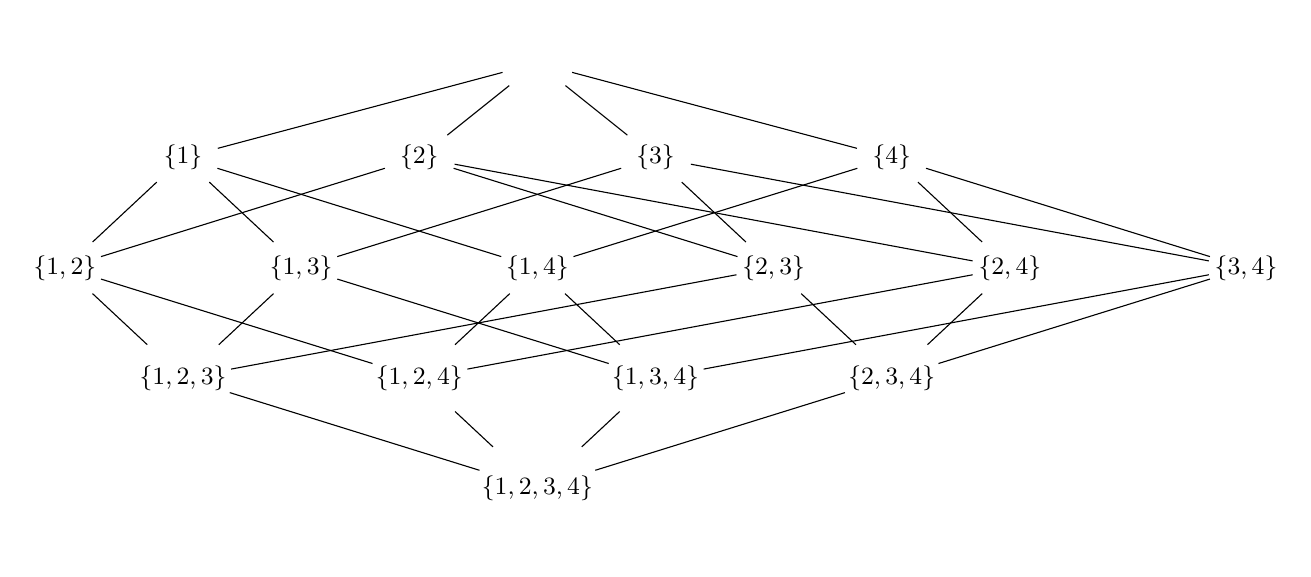
\begin{tikzpicture}[
                every node/.style={inner sep=1pt, font=\small},
                lvl/.style={yshift=#1},
                dot/.style={circle, minimum size=9mm},
                >=stealth
            ]
            % لایه 0
            \node[dot] (e) {$\varnothing$};

            % لایه 1
            \node[dot, lvl=-1.2cm, xshift=-4.5cm] (1) {$\{1\}$};
            \node[dot, lvl=-1.2cm, xshift=-1.5cm] (2) {$\{2\}$};
            \node[dot, lvl=-1.2cm, xshift= 1.5cm] (3) {$\{3\}$};
            \node[dot, lvl=-1.2cm, xshift= 4.5cm] (4) {$\{4\}$};

            % لایه 2
            \node[dot, lvl=-2.6cm, xshift=-6.0cm] (12) {$\{1,2\}$};
            \node[dot, lvl=-2.6cm, xshift=-3.0cm] (13) {$\{1,3\}$};
            \node[dot, lvl=-2.6cm, xshift= 0.0cm] (14) {$\{1,4\}$};
            \node[dot, lvl=-2.6cm, xshift= 3.0cm] (23) {$\{2,3\}$};
            \node[dot, lvl=-2.6cm, xshift= 6.0cm] (24) {$\{2,4\}$};
            \node[dot, lvl=-2.6cm, xshift= 9.0cm] (34) {$\{3,4\}$};

            % لایه 3
            \node[dot, lvl=-4.0cm, xshift=-4.5cm] (123) {$\{1,2,3\}$};
            \node[dot, lvl=-4.0cm, xshift=-1.5cm] (124) {$\{1,2,4\}$};
            \node[dot, lvl=-4.0cm, xshift= 1.5cm] (134) {$\{1,3,4\}$};
            \node[dot, lvl=-4.0cm, xshift= 4.5cm] (234) {$\{2,3,4\}$};

            % لایه 4
            \node[dot, lvl=-5.4cm] (1234) {$\{1,2,3,4\}$};

            % یال‌ها (روابط پوشا)


            \draw (e) -- (1) (e) -- (2) (e) -- (3) (e) -- (4);

            \draw (1) -- (12) (1) -- (13) (1) -- (14);
            \draw (2) -- (12) (2) -- (23) (2) -- (24);
            \draw (3) -- (13) (3) -- (23) (3) -- (34);
            \draw (4) -- (14) (4) -- (24) (4) -- (34);

            \draw (12) -- (123) (12) -- (124);
            \draw (13) -- (123) (13) -- (134);
            \draw (14) -- (124) (14) -- (134);
            \draw (23) -- (123) (23) -- (234);
            \draw (24) -- (124) (24) -- (234);
            \draw (34) -- (134) (34) -- (234);

            \draw (123) -- (1234);
            \draw (124) -- (1234);
            \draw (134) -- (1234);
            \draw (234) -- (1234);
        \end{tikzpicture}
    }
\end{frame}



\begin{frame}[t]{عنصر ماکسیمال}

    \begin{definition}
        فرض کنید $(A,\le)$ یک مجموعهٔ مرتبِ جزئی باشد. عنصری $a\in A$ را \textit{بیشینه (ماکسیمال) در $A$} می‌نامیم هرگاه برای هر $c\in A$ که \textit{با $a$ قابلِ مقایسه} است، داشته باشیم $c\le a$؛ به‌عبارتِ دیگر، برای همهٔ $c\in A$،
        \[
            a \le c \;\Rightarrow\; a = c.
        \]
    \end{definition}



\end{frame}

\begin{frame}[t,fragile]{نمونه‌هایی از عناصر ماکسیمال}
    توجه کنید اگر $a$ بیشینه باشد، الزاماً این‌گونه نیست که برای همهٔ $c\in A$ داشته باشیم $c\le a$ (ممکن است عناصری در $A$ باشند که با $a$ قابلِ مقایسه نباشند). همچنین یک مجموعه ممکن است چندین عنصرِ بیشینه داشته باشد، یا اصلاً هیچ عنصری بیشینه نداشته باشد (برای مثال، $\mathbb{Z}$ با ترتیبِ معمولش).



    \begin{example}
        \centering
        \resizebox{0.78\linewidth}{!}{
            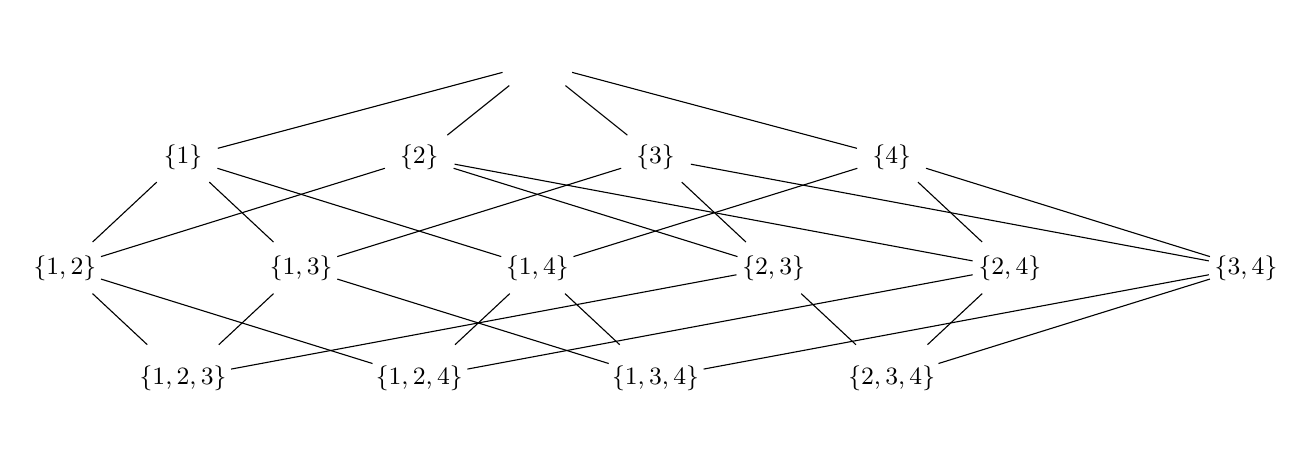
\begin{tikzpicture}[
                    every node/.style={inner sep=1pt, font=\small},
                    lvl/.style={yshift=#1},
                    dot/.style={circle, minimum size=9mm},
                    >=stealth
                ]
                % لایه 0
                \node[dot] (e) {$\varnothing$};

                % لایه 1
                \node[dot, lvl=-1.2cm, xshift=-4.5cm] (1) {$\{1\}$};
                \node[dot, lvl=-1.2cm, xshift=-1.5cm] (2) {$\{2\}$};
                \node[dot, lvl=-1.2cm, xshift= 1.5cm] (3) {$\{3\}$};
                \node[dot, lvl=-1.2cm, xshift= 4.5cm] (4) {$\{4\}$};

                % لایه 2
                \node[dot, lvl=-2.6cm, xshift=-6.0cm] (12) {$\{1,2\}$};
                \node[dot, lvl=-2.6cm, xshift=-3.0cm] (13) {$\{1,3\}$};
                \node[dot, lvl=-2.6cm, xshift= 0.0cm] (14) {$\{1,4\}$};
                \node[dot, lvl=-2.6cm, xshift= 3.0cm] (23) {$\{2,3\}$};
                \node[dot, lvl=-2.6cm, xshift= 6.0cm] (24) {$\{2,4\}$};
                \node[dot, lvl=-2.6cm, xshift= 9.0cm] (34) {$\{3,4\}$};

                % لایه 3
                \node[dot, lvl=-4.0cm, xshift=-4.5cm] (123) {$\{1,2,3\}$};
                \node[dot, lvl=-4.0cm, xshift=-1.5cm] (124) {$\{1,2,4\}$};
                \node[dot, lvl=-4.0cm, xshift= 1.5cm] (134) {$\{1,3,4\}$};
                \node[dot, lvl=-4.0cm, xshift= 4.5cm] (234) {$\{2,3,4\}$};

                % یال‌ها (روابط پوشا)


                \draw (e) -- (1) (e) -- (2) (e) -- (3) (e) -- (4);

                \draw (1) -- (12) (1) -- (13) (1) -- (14);
                \draw (2) -- (12) (2) -- (23) (2) -- (24);
                \draw (3) -- (13) (3) -- (23) (3) -- (34);
                \draw (4) -- (14) (4) -- (24) (4) -- (34);

                \draw (12) -- (123) (12) -- (124);
                \draw (13) -- (123) (13) -- (134);
                \draw (14) -- (124) (14) -- (134);
                \draw (23) -- (123) (23) -- (234);
                \draw (24) -- (124) (24) -- (234);
                \draw (34) -- (134) (34) -- (234);


            \end{tikzpicture}
        }


    \end{example}

    \begin{example}
        \centering
        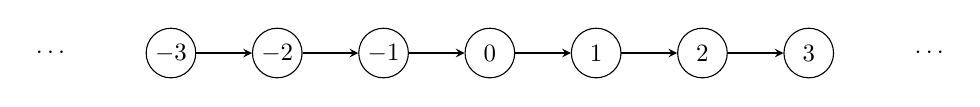
\begin{tikzpicture}[>=stealth, scale=0.9, transform shape]
            % points:  ... -3, -2, -1, 0, 1, 2, 3 ...
            \node (dotsL) at (-6.2,0) {$\cdots$};
            \node[circle, draw, minimum size=7mm, inner sep=1pt] (m3) at (-4.5,0) {$-3$};
            \node[circle, draw, minimum size=7mm, inner sep=1pt] (m2) at (-3.0,0) {$-2$};
            \node[circle, draw, minimum size=7mm, inner sep=1pt] (m1) at (-1.5,0) {$-1$};
            \node[circle, draw, minimum size=7mm, inner sep=1pt] (z0) at (0,0) {$0$};
            \node[circle, draw, minimum size=7mm, inner sep=1pt] (p1) at (1.5,0) {$1$};
            \node[circle, draw, minimum size=7mm, inner sep=1pt] (p2) at (3.0,0) {$2$};
            \node[circle, draw, minimum size=7mm, inner sep=1pt] (p3) at (4.5,0) {$3$};
            \node (dotsR) at (6.2,0) {$\cdots$};

            % cover relations (arrows point to the greater element)
            \begin{scope}[->]
                \draw (m3) -- (m2);
                \draw (m2) -- (m1);
                \draw (m1) -- (z0);
                \draw (z0) -- (p1);
                \draw (p1) -- (p2);
                \draw (p2) -- (p3);
            \end{scope}
        \end{tikzpicture}
    \end{example}


\end{frame}


\begin{frame}[t]{کران بالا و زنجیر}
    \begin{definition}
        یک \textit{کران بالا} برای زیرمجموعه‌ای ناتهی $B$ از $A$ عنصری $d \in A$ است به‌طوری‌که
        \[
            \forall b \in B; \quad b \le d
        \]


    \end{definition}

    \begin{definition}
        زیرمجموعهٔ ناتهی $B$ از $A$ که به‌وسیلهٔ رابطهٔ $\le$ به‌صورت خطی مرتب شده باشد، یک \textit{زنجیر در $A$} نامیده می‌شود.
    \end{definition}



\end{frame}

\begin{frame}[t]{لم زورن}

    \begin{definition}[لم زورن ]
        اگر $A$ یک مجموعهٔ مرتبِ جزئیِ ناتهی باشد به‌طوری‌که هر زنجیر در $A$ دارای کرانِ بالا در $A$ باشد، آنگاه $A$ دارای عنصری بیشینه است.
    \end{definition}


    با فرضِ این‌که سایر اصولِ موضوعهٔ معمولِ نظریهٔ مجموعه‌ها برقرارند، می‌توان اثبات کرد که لمِ زورن درست است اگر و تنها اگر اصلِ انتخاب برقرار باشد؛ به‌عبارتِ دیگر، این دو با یکدیگر \textit{معادل‌اند.}

\end{frame}
\standout{تمرین}
\begin{frame}[t]{لتیس و کران‌های پایین و بالا}
    \begin{exercise}
        فرض کنید $(A,\le)$ یک مجموعهٔ مرتبِ جزئی باشد و $B$ زیرمجموعه‌ای ناتهی. یک \textit{کرانِ پایین} برای $B$ عنصری $d \in A$ است به‌طوری‌که برای \textit{هر} $b \in B$ داشته باشیم $d \le b$. یک \textit{بزرگ‌ترین کرانِ پایین \lr{(g.l.b.)}} برای $B$ کرانِ پایینی $d_0$ از $B$ است به‌گونه‌ای که برای هر کرانِ پایینِ دیگرِ $d$ از $B$ داشته باشیم $d \le d_0$. یک \textit{کوچک‌ترین کرانِ بالا \lr{(l.u.b.)}} برای $B$ کرانِ بالایی $t_0$ از $B$ است به‌گونه‌ای که برای هر کرانِ بالایِ دیگرِ $t$ داشته باشیم $t_0 \le t$. زوجِ $(A,\le)$ یک \textit{لتیس} است هرگاه برای همۀ $a,b \in A$ مجموعهٔ $\{a,b\}$ هم بزرگ‌ترین کرانِ پایین و هم کوچک‌ترین کرانِ بالا را داشته باشد.

        \begin{enumerate}
            \item اگر $S \ne \emptyset$، آنگاه توانِ مجموعهٔ $\mathcal{P}(S)$ با ترتیبِ شمولِ مجموعه‌ای یک لتیس است که یک عنصرِ بیشینهٔ یکتا دارد.
            \item مثالی از یک مجموعهٔ مرتبِ جزئی بیاورید که \textit{لتیس نباشد}.
            \item مثالی از یک لتیس بدونِ عنصرِ بیشینه و نیز مثالی از یک مجموعهٔ مرتبِ جزئی با دو عنصرِ بیشینه بیاورید.
        \end{enumerate}

    \end{exercise}
\end{frame}

\begin{frame}[t]{لتیس کامل و نقطهٔ ثابت}

    \begin{exercise}
        یک لتیس $(A,\le)$ (بنگرید به تمرین~1) را \textit{کامل} می‌نامیم هرگاه هر زیرمجموعهٔ ناتهی از $A$ هم کوچک‌ترین کرانِ بالا و هم بزرگ‌ترین کرانِ پایین را داشته باشد.
        تابعی میان مجموعه‌های مرتبِ جزئی $f\colon A \to B$ را \textit{حافظِ ترتیب} می‌نامیم هرگاه از $a \le a'$ در $A$ نتیجه شود که $f(a) \le f(a')$ در $B$.
        اثبات کنید که یک تابعِ حافظِ ترتیب $f$ از یک لتیس کاملِ $A$ به خودش، دست‌کم یک عنصرِ ثابت دارد (یعنی عنصری $a \in A$ که $f(a)=a$).

    \end{exercise}

    \begin{exercise}
        یک ترتیبِ خوش‌ترتیب بر مجموعهٔ اعدادِ گویا $\mathbb{Q}$ ارائه دهید.

    \end{exercise}
\end{frame}



\begin{frame}[t]{تابع انتخاب و ترتیب در صفحه}
    \begin{exercise}
        فرض کنید $S$ یک مجموعه باشد. یک \textit{تابعِ انتخاب برای $S$} تابعی است
        \( f \) از مجموعهٔ تمام زیرمجموعه‌های ناتهیِ $S$ به $S$، یعنی
        \[
            f:\{\,A \subseteq S \mid A \neq \emptyset\,\}\longrightarrow S,
        \]
        به‌طوری‌که برای هر \( A \neq \emptyset \) با \( A \subseteq S \) داشته باشیم \( f(A)\in A \).
        نشان دهید که «اصلِ انتخاب» معادلِ این گزاره است که هر مجموعهٔ \( S \) دارای یک تابعِ انتخاب است.

    \end{exercise}

\end{frame}

\begin{frame}[t]{ترتیبی با بی‌نهایت عنصر ماکسیمال}
    \begin{exercise}
        فرض کنید $S$ مجموعهٔ همهٔ نقاط $(x,y)$ در صفحه باشد که $y \le 0$. ترتیبی به‌صورت
        \[
            (x_1,y_1) \le (x_2,y_2) \;\Leftrightarrow\; x_1 = x_2 \ \text{و}\ y_1 \le y_2
        \]
        تعریف می‌کنیم. نشان دهید که این یک ترتیبِ جزئی بر $S$ است و این‌که $S$ بی‌نهایت عنصرِ بیشینه دارد.

    \end{exercise}


\end{frame}
